\documentclass[journal,12pt,twocolumn]{IEEEtran}

\usepackage{setspace}
\usepackage{gensymb}
\singlespacing
\usepackage[cmex10]{amsmath}

\usepackage{amsthm}

\usepackage{mathrsfs}
\usepackage{txfonts}
\usepackage{amsmath}
\usepackage{stfloats}
\usepackage{float}
\usepackage{bm}
\usepackage{tikz}
\usepackage{pgfplots}
\usepackage{cite}
\usepackage{cases}
\usepackage{subfig}

\usepackage{longtable}
\usepackage{multirow}

\usepackage{enumitem}
\usepackage{mathtools}
\usepackage{steinmetz}
\usepackage{tikz}
\usepackage{circuitikz}
\usepackage{verbatim}
\usepackage{tfrupee}
\usepackage[breaklinks=true]{hyperref}
\usepackage{graphicx}
\usepackage{tkz-euclide}

\usetikzlibrary{calc,math}
\usetikzlibrary{shapes.geometric, arrows}
\usepackage{listings}
    \usepackage{color}                                            %%
    \usepackage{array}                                            %%
    \usepackage{longtable}                                        %%
    \usepackage{calc}                                             %%
    \usepackage{multirow}                                         %%
    \usepackage{hhline}                                           %%
    \usepackage{ifthen}                                           %%
    \usepackage{lscape}
\usepackage{multicol}
\usepackage{chngcntr}
\usepackage{hyperref}
\hypersetup{
    colorlinks=true,
    linkcolor=blue,
    filecolor=blue,
    urlcolor=blue,
}
\DeclareMathOperator*{\Res}{Res}
\DeclareMathOperator{\sinc}{sinc}
\DeclareMathOperator{\rect}{rect}

\renewcommand\thesection{\arabic{section}}
\renewcommand\thesubsection{\thesection.\arabic{subsection}}
\renewcommand\thesubsubsection{\thesubsection.\arabic{subsubsection}}

\renewcommand\thesectiondis{\arabic{section}}
\renewcommand\thesubsectiondis{\thesectiondis.\arabic{subsection}}
\renewcommand\thesubsubsectiondis{\thesubsectiondis.\arabic{subsubsection}}


\hyphenation{op-tical net-works semi-conduc-tor}
\def\inputGnumericTable{}                                 %%

\lstset{
%language=C,
frame=single,
breaklines=true,
columns=fullflexible
}

\makeatletter
\setlength{\@fptop}{0pt}
\makeatother

\begin{document}


\newtheorem{theorem}{Theorem}[section]
\newtheorem{problem}{Problem}
\newtheorem{proposition}{Proposition}[section]
\newtheorem{lemma}{Lemma}[section]
\newtheorem{corollary}[theorem]{Corollary}
\newtheorem{example}{Example}[section]
\newtheorem{definition}[problem]{Definition}

\newcommand{\BEQA}{\begin{eqnarray}}
\newcommand{\EEQA}{\end{eqnarray}}
\newcommand{\define}{\stackrel{\triangle}{=}}
\newcommand*\Eval[3]{\left.#1\right\rvert_{#2}^{#3}}
\bibliographystyle{IEEEtran}
\raggedbottom
\setlength{\parindent}{0pt}
\providecommand{\mbf}{\mathbf}
\providecommand{\pr}[1]{\ensuremath{\Pr\left(#1\right)}}
\providecommand{\qfunc}[1]{\ensuremath{Q\left(#1\right)}}
\providecommand{\sbrak}[1]{\ensuremath{{}\left[#1\right]}}
\providecommand{\lsbrak}[1]{\ensuremath{{}\left[#1\right.}}
\providecommand{\rsbrak}[1]{\ensuremath{{}\left.#1\right]}}
\providecommand{\brak}[1]{\ensuremath{\left(#1\right)}}
\providecommand{\lbrak}[1]{\ensuremath{\left(#1\right.}}
\providecommand{\rbrak}[1]{\ensuremath{\left.#1\right)}}
\providecommand{\cbrak}[1]{\ensuremath{\left\{#1\right\}}}
\providecommand{\lcbrak}[1]{\ensuremath{\left\{#1\right.}}
\providecommand{\rcbrak}[1]{\ensuremath{\left.#1\right\}}}
\theoremstyle{remark}
\newtheorem{rem}{Remark}
\newcommand{\sgn}{\mathop{\mathrm{sgn}}}
\providecommand{\abs}[1]{$\left\vert#1\right\vert$}
\providecommand{\res}[1]{\Res\displaylimits_{#1}}
\providecommand{\norm}[1]{$\left\lVert#1\right\rVert$}
%\providecommand{\norm}[1]{\lVert#1\rVert}
\providecommand{\mtx}[1]{\mathbf{#1}}
\providecommand{\mean}[1]{$E\left[ #1 \right]$}
\providecommand{\fourier}{\overset{\mathcal{F}}{ \rightleftharpoons}}
%\providecommand{\hilbert}{\overset{\mathcal{H}}{ \rightleftharpoons}}
\providecommand{\system}{\overset{\mathcal{H}}{ \longleftrightarrow}}
	%\newcommand{\solution}[2]{\textbf{Solution:}{#1}}
\newcommand{\solution}{\noindent \textbf{Solution: }}
\newcommand{\cosec}{\,\text{cosec}\,}
\providecommand{\dec}[2]{\ensuremath{\overset{#1}{\underset{#2}{\gtrless}}}}
\newcommand{\myvec}[1]{\ensuremath{\begin{pmatrix}#1\end{pmatrix}}}
\newcommand{\mydet}[1]{\ensuremath{\begin{vmatrix}#1\end{vmatrix}}}
\newcommand*{\permcomb}[4][0mu]{{{}^{#3}\mkern#1#2_{#4}}}
\newcommand*{\perm}[1][-3mu]{\permcomb[#1]{P}}
\newcommand*{\comb}[1][-1mu]{\permcomb[#1]{C}}
\numberwithin{equation}{subsection}
\makeatletter
\@addtoreset{figure}{problem}
\makeatother
\let\StandardTheFigure\thefigure
\let\vec\mathbf
\renewcommand{\thefigure}{\theproblem}
\def\putbox#1#2#3{\makebox[0in][l]{\makebox[#1][l]{}\raisebox{\baselineskip}[0in][0in]{\raisebox{#2}[0in][0in]{#3}}}}
     \def\rightbox#1{\makebox[0in][r]{#1}}
     \def\centbox#1{\makebox[0in]{#1}}
     \def\topbox#1{\raisebox{-\baselineskip}[0in][0in]{#1}}
     \def\midbox#1{\raisebox{-0.5\baselineskip}[0in][0in]{#1}}
\vspace{3cm}
\title{GATE Assignment 1}
\author{Perambuduri Srikaran - AI20BTECH11018}
\maketitle
\newpage
\bigskip
\renewcommand{\thefigure}{\theenumi}
\renewcommand{\thetable}{\theenumi}
Download all python codes from
\begin{lstlisting}
https://github.com/srikaran-p/AI1103/tree/main/GATE_Assignment1/codes
\end{lstlisting}
Download all latex codes from
\begin{lstlisting}
https://github.com/srikaran-p/EE3900/tree/main/GATE_Assignment1
\end{lstlisting}
\section*{Problem}
(GATE EC-2018 Q.39) The input $4\sinc{\brak{2t}}$ is fed to a Hilbert transformer to obtain $y\brak{t}$, as shown in the figure below:
\tikzstyle{noborder} = [rectangle, draw=none, fill=white!50,
    text centered, rounded corners, minimum height=2em]
\tikzstyle{block} = [rectangle, draw, fill=white!50,
    text width=4.5em, text centered, minimum height=2em]
\tikzstyle{line} = [draw, -latex']
\begin{center}
\begin{tikzpicture}
[node distance = 2.8cm, auto]
    \node [noborder] (init){$4\sinc{\brak{2t}}$};
    \node [block, right of = init] (transformer){Hilbert Transform};
    \node [noborder, right of = transformer] (result){$y\brak{t}$};

     \path [line] (init) -- (transformer);
     \path [line] (transformer) -- (result);
\end{tikzpicture}
\end{center}
Here, $\sinc{\brak{x}} = \frac{\sin\brak{\pi x}}{\pi x}$. The value (accurate to two decimal places) of $\int_{-\infty}^{\infty} |y\brak{t}|^2 dt$ is
\section*{Solution}
\begin{lemma}
Parseval's theorem states that there is no loss of information in Fourier transform and the amount of energy remains the same in time and frequency domains.
\begin{align}
    \int_{-\infty}^{\infty} |x\brak{t}|^{2} dt = \int_{-\infty}^{\infty} |X\brak{f}|^{2} df
\end{align}
\end{lemma}
\begin{align}
    x(t) &= 4\sinc(2t)\\
    h(t) &= \frac{1}{\pi t}\\
    y(t) &= x(t) * h(t) \label{eq:1}\\
    x(t) &\fourier{X(f)}\\
    h(t) &\fourier{H(f)}\\
    y(t) &\fourier{Y(f)}
\end{align}
Define a rectangular function,
\begin{align}
    \rect(t) =
    \begin{cases}
    1 & \text{if } |t| \leq 1\\
    0 & \text{if } |t| > 1
    \end{cases}
\end{align}
Define a signum function,
\begin{align}
    \sgn(t) =
    \begin{cases}
    1 & \text{if } t > 0\\
    0 & \text{if } t = 0\\
    -1 & \text{if } t < 0
    \end{cases}
\end{align}
The Fourier transforms are
\begin{align}
    X(f) &= 2\rect(f)\\
    H(f) &= -j\sgn(f)
\end{align}
Applying Convolution theorem in \eqref{eq:1},
\begin{align}
    Y(f) &= X(f)H(f)\\
    &= -2j\rect(f)\sgn(f)
\end{align}
Applying Inverse Fourier Transform on $Y(f)$,
\begin{align}
    y(t) &= \int_{-\infty}^{\infty} Y(f)e^{j2\pi ft}df\\
    &= \int_{-1}^{0} 2je^{j2\pi ft}df + \int_{0}^{1} -2je^{j2\pi ft}df\\
    &= \frac{2j}{j2\pi t}e^{j2\pi ft}\Biggr|_{-1}^{0} - \frac{2j}{j2\pi t}e^{j2\pi ft}\Biggr|_{0}^{1}\\
    &= \frac{2}{\pi t} -\frac{1}{\pi t}e^{-j2\pi t} - \frac{1}{\pi t}e^{j2\pi t}\\
    &= \frac{2}{\pi t} - \frac{2cos(\pi t)}{\pi t}\\
    &= \frac{2}{\pi t}\brak{1 - cos(\pi t)}
\end{align}
By the Parseval's theorem,
\begin{align}
    \int_{-\infty}^{\infty} |y\brak{t}|^{2} dt &= \int_{-\infty}^{\infty} |Y\brak{f}|^{2} df\\
    &= \int_{-1}^{1} |2rect(f)|^2df\\
    &= 8
\end{align}
\begin{figure}[htp]
    \centering
    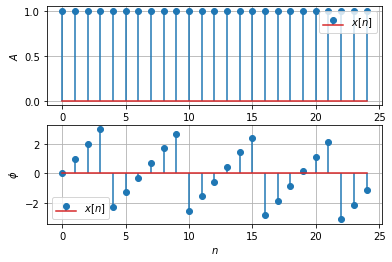
\includegraphics[width=\columnwidth]{Fig1.png}
    \caption{Input and Output Signals}
    \label{fig:plot}
\end{figure}
\end{document}
